\documentclass{Beautybook-V6.1}
\usepackage{rotating}
\tikzset{>=Stealth}
\setlist{nosep,font=\upshape} % 取消所有列表默认距离
% 浮动环境设置
% 默认情况下, \LaTeX{} 要求每页的文字至少占据 20%,否则该页就只单独放置一个浮动环境,
% 而这通常不是我们想要的, 我们将这个要求降低到 5%.
\renewcommand*{\textfraction}{0.05}
% 有时如果多个浮动环境连续放在一起,
% 会将它们分在几个不同页,即使它们可在同一页放
% 得下. 我们可以通过修改 |\topfraction| 和 |\bottomfraction| 分别设置顶端和底端的浮
% 动环境的最大比例.
\renewcommand*{\topfraction}{0.9}
\renewcommand*{\bottomfraction}{0.8}
% 有时\LaTeX{}会把一个浮动环境单独放在一页,
% 我们要求这个环境至少要占据 85% 才能单独放在一页.
% 注意:  |\floatpagefraction| 的数值必须小于 |\topfraction|.
\renewcommand*{\floatpagefraction}{0.85}
% 关于图片 graphicx
% 如果图片没有指定后缀, 依次按下列顺序搜索
\DeclareGraphicsExtensions{.pdf,.eps,.jpg,.png}
% 设置图表搜索路径, 可以给图表文件夹取如下名字
\graphicspath{{figures/}{figure/}{pictures/}{picture/}{pic/}{pics/}{image/}{images/}}
\usepackage{mtpro2}
\usepackage[physics]{stys/physicx}
\usepackage{stys/Symbols}
\usepackage{amsfonts}
\DeclareFontFamily{U}{nxlmi}{}
\DeclareFontSubstitution{U}{nxlmi}{m}{it}
\DeclareFontShape{U}{nxlmi}{m}{it}{
<-6.3>    nxlmi05
<6.3-8.6> nxlmi07
<8.6->    nxlmi0
}{}

\DeclareFontShape{U}{nxlmi}{b}{it}{
<-6.3>    nxlbmi05
<6.3-8.6> nxlbmi07
<8.6->    nxlbmi0
}{}

\renewcommand{\partial}{{\text{\usefont{U}{nxlmi}{m}{it}\symbol{64}}\mspace{1mu}}}

%% 定义第一种定理
\mynewtheorem{
    defi={\textbf{定义}}[section]{interior style={left color=ReD!8,right color=ReD!5!CyaN!50}, borderline west={1.5mm}{0mm}{ReD}},
    thm={\textbf{定理}}[section]{interior style={left color=CyaN!80!black!20,right color=CyaN!80!black!15!CyaN!50}, borderline west={1.5mm}{0mm}{CyaN!80!black}},
    lem={\textbf{引理}}[section]{interior style={left color=BluE!8,right color=BluE!5!CyaN!50}, borderline west={1.5mm}{0mm}{BluE}},
    prop={\textbf{命题}}[section]{interior style={left color=OrangE!8,right color=OrangE!5!CyaN!50}, borderline west={1.5mm}{0mm}{OrangE}},
    exam={\textbf{题}}[chapter]{interior style={left color=DarkGreen!8,right color=DarkGreen!5!CyaN!50}, borderline west={1.5mm}{0mm}{DarkGreen}},
    cor={\textbf{推论}}[chapter]{interior style={left color=violet!8,right color=violet!5!CyaN!50}, borderline west={1.5mm}{0mm}{violet}},
}
\newtheorem*{remark}{\textbf{注}}
%% 定义第二种定理
% overlay unbroken=\my@theorem@overlay@unbroken{\theorem@name\ \thetcbthm}{额外的选项}
% overlay first=\my@theorem@overlay@first{\theorem@name\ \thetcbthm}{额外的选项}
%% 用户接口区
\definecolor{examback}{HTML}{e3e6e8}
\makeatletter
\mynewtcbtheorem{
    % 这个 theorem 是环境名
    theorem={
        counter=tcbthm, 
        the counter=\thesection.\arabic{tcbthm}, 
        name=定理, % 它保存到 \theorem@name 里
        thmcolor=purple5,
        autoref name=\bfseries 定理, 
        style={
        arc=3pt,breakable,enhanced,interior style={top color=purple5!5 ,middle color=purple5!1!nuanbai, bottom color=nuanbai},boxrule=0pt,top=8mm,
        fuzzy shadow={-0.6mm}{0.6mm}{0mm}{0.3mm}{white!50!gray},% 上
        fuzzy shadow={0.6mm}{-0.6mm}{0mm}{0.3mm}{fill=white!40!gray},%下
        opacityframe=0, opacityback=0.98,
        fontupper=\itshape, step={tcbthm},
        before pre=\smallskip, after app=\smallskip,
        overlay unbroken=\my@theorem@overlay@unbroken{\theorem@name\ \thetcbthm}{\theorem@thmcolor},
        overlay first=\my@theorem@overlay@first{\theorem@name\ \thetcbthm}{\theorem@thmcolor},
        overlay last=\my@theorem@overlay@last{\theorem@thmcolor},
        }
    },
    proposition={
        counter=tcbprop, 
        the counter=\thesection.\arabic{tcbprop}, 
        autoref name=\bfseries 命题, 
        style={
        arc=3pt,breakable,enhanced,interior style={top color=DeepPink!5 ,middle color=DeepPink!1!nuanbai, bottom color=nuanbai},boxrule=0pt,top=8mm,
        fuzzy shadow={-0.6mm}{0.6mm}{0mm}{0.3mm}{white!50!gray},% 上
        fuzzy shadow={0.6mm}{-0.6mm}{0mm}{0.3mm}{fill=white!40!gray},%下
        opacityframe=0, opacityback=0.98,
        fontupper=\itshape, step={tcbprop},
        before pre=\smallskip, after app=\smallskip,
        overlay unbroken=\my@theorem@overlay@unbroken{命题\ \thetcbprop}{DeepPink},
        overlay first=\my@theorem@overlay@first{命题\ \thetcbprop}{DeepPink},
        overlay last=\my@theorem@overlay@last{DeepPink},
        }
    },
    definition={
        counter=tcbdefi, 
        the counter=\thesection.\arabic{tcbdefi}, 
        autoref name=\bfseries 定义, 
        style={
        arc=3pt,breakable,enhanced,interior style={top color=紫棠!5 ,middle color=紫棠!1!nuanbai, bottom color=nuanbai},boxrule=0pt,top=8mm,
        fuzzy shadow={-0.6mm}{0.6mm}{0mm}{0.3mm}{white!50!gray},% 上
        fuzzy shadow={0.6mm}{-0.6mm}{0mm}{0.3mm}{fill=white!40!gray},%下
        opacityframe=0, opacityback=0.98,
        fontupper=\itshape, step={tcbdefi},
        before pre=\smallskip, after app=\smallskip,
        overlay unbroken=\my@theorem@overlay@unbroken{定义\ \thetcbdefi}{紫棠},
        overlay first=\my@theorem@overlay@first{定义\ \thetcbdefi}{紫棠},
        overlay last=\my@theorem@overlay@last{紫棠},
        }
    },
    lemma={
        counter=tcblem,
        the counter=\thesection.\arabic{tcblem},
        name=引理, 
        lemcolor=靛蓝, 
        autoref name=\bfseries 引理,
        style={
        arc=0mm,breakable,enhanced,interior style={top color=靛蓝!5 ,middle color=靛蓝!1!nuanbai, bottom color=nuanbai},arc=3pt,boxrule=0pt,top=7mm,bottom=5mm,
        fuzzy shadow={-0.6mm}{0.6mm}{0mm}{0.3mm}{white!50!gray},% 上
        fuzzy shadow={0.6mm}{-0.6mm}{0mm}{0.3mm}{fill=white!40!gray},%下
        opacityframe=0, opacityback=0.98,
        fontupper=\normalsize,step={tcblem},
        before pre=\smallskip, after app=\smallskip,
        overlay unbroken=\my@lemma@overlay@unbroken{\lemma@name\ \thetcblem}{\lemma@lemcolor},
        overlay first=\my@lemma@overlay@first{\lemma@name\ \thetcblem}{\lemma@lemcolor},
        overlay last=\my@lemma@overlay@last{\lemma@lemcolor},
        }
    },
    corollary={
        counter=tcbcor,
        the counter=\thesection.\arabic{tcbcor},
        autoref name=\bfseries 推论,
        style={
        arc=0mm,breakable,enhanced,interior style={top color=茶色!5 ,middle color=茶色!1!nuanbai, bottom color=nuanbai},arc=3pt,boxrule=0pt,top=7mm,bottom=5mm,
        fuzzy shadow={-0.6mm}{0.6mm}{0mm}{0.3mm}{white!50!gray},% 上
        fuzzy shadow={0.6mm}{-0.6mm}{0mm}{0.3mm}{fill=white!40!gray},%下
        opacityframe=0, opacityback=0.98,
        fontupper=\normalsize,step={tcbcor},
        before pre=\smallskip, after app=\smallskip,
        overlay unbroken=\my@lemma@overlay@unbroken{推论\ \thetcbcor}{茶色},
        overlay first=\my@lemma@overlay@first{推论\ \thetcbcor}{茶色},
        overlay last=\my@lemma@overlay@last{茶色},
        }
    },
    example={
        counter=tcbexam,
        the counter=\thesection.\arabic{tcbexam},
        autoref name=\bfseries 例题,
        style={
        arc=0mm,breakable,enhanced,interior style={top color=黛绿!5 ,middle color=黛绿!1!nuanbai, bottom color=nuanbai},arc=3pt,boxrule=0pt,top=7mm,bottom=5mm,
        fuzzy shadow={-0.6mm}{0.6mm}{0mm}{0.3mm}{white!50!gray},% 上
        fuzzy shadow={0.6mm}{-0.6mm}{0mm}{0.3mm}{fill=white!40!gray},%下
        opacityframe=0, opacityback=0.98,
        fontupper=\normalsize,step={tcbexam},
        before pre=\smallskip, after app=\smallskip,
        overlay unbroken=\my@lemma@overlay@unbroken{例题\ \thetcbexam}{黛绿},
        overlay first=\my@lemma@overlay@first{例题\ \thetcbexam}{黛绿},
        overlay last=\my@lemma@overlay@last{黛绿},
        }
    },
}
\makeatother
\newenvironment{note}[1][\bf 笔记:]{\Line\uuline{#1} }{\Line}
\renewcommand{\Line}{\noindent\\\tikz\draw[line width=0.65pt,gray!80,dashed] (0,0)--++(.99\linewidth,0);\par}
\newenvironment{key}[1][]{\begin{fancybox}{#1}}{\end{fancybox}}
\newcommand{\Diff}[2][]{\frac{\partial #1}{\partial #2}}
\newcommand{\Dif}[2]{\frac{\dd #1}{\dd #2}}
\newcommand{\pr}{^\prime}
\usepackage{extarrows}
\usetikzlibrary{tikzmark}
% \arrowname{super-script}
% \arrowname[sub-script]{super-script}
\begin{document}
\thispagestyle{empty}
\title{Reviewing Material}
\subtitle{信息技术学考导引试题详解}
\edition{First Edition}
\bookseries{Preperation For The Final Test}
\author{xaero}
\pressname{}
\presslogo{figures/hglogo.pdf}
\coverimage{figures/pexels-alex-andrews-816608.jpg}
\makecover

\definecolor{bg}{HTML}{e0e0e0}
\definecolor{fg}{HTML}{455a64}
\colorlet{outermarginbgcolor}{bg}
\colorlet{outermarginfgcolor}{fg}
\colorlet{framegolden}{fg}
\colorlet{framegray}{黛绿!5}

\thispagestyle{empty}
\begin{titlepage}
\thispagestyle{empty}
    \begin{center}
    
    %% Print the bookseries
    {\makeatletter\vspace*{5mm}
    \ifdefvoid{\@bookseries}{}{\bigskip\normalfont\fontsize{20}{20}\selectfont\@bookseries}
    \makeatother}

        \bigskip
        \bigskip

    %% Print the title
    {\makeatletter
    \fontsize{18}{20}\rmfamily\selectfont\@title \\\vspace*{5mm}
    \fontsize{32}{35}\rmfamily\bfseries\selectfont 2023信息技术学考导引试题详解
    \makeatother}
    
    \bigskip
    \bigskip
    
    \bigskip
    \bigskip
    \bigskip

    %% Print the name of the author
    {\makeatletter
    \fontsize{16}{25}\rmfamily\selectfont 陈\hspace{5mm}功\hspace{5mm}杰
    \makeatother}
    
    \bigskip
    \bigskip

    
    \vfill
    
    
    \bigskip
    \bigskip
    
    {\makeatletter
    %\fontsize{25}{25}\rmfamily\selectfont\@pressname
    \vspace*{-5mm}
    \centering
    
\includegraphics[width=0.4\linewidth]{figures/hglogoblack}    
    \makeatother}
    \end{center}
    
    \end{titlepage}
    \let\cleardoublepage\clearpage

    \thispagestyle{empty}
    \begin{center}
        {
        \vspace*{5cm}
        \fontsize{14}{20}\rmfamily\selectfont    源\hspace{1em}码\hspace{1em}获\hspace{1em}取}\\ 
        \bigskip
        \bigskip
        \href{https://github.com/xaero7/HG_DaoYin}{https://github.com/xaero7/HG\_DaoYin}


    \end{center}







\frontmatter
\pagenumbering{Roman}
%\input{chapters/preface}
\thispagestyle{empty}
\tableofcontents\let\cleardoublepage\clearpage

\mainmatter
\pagenumbering{arabic}
\partimage{figures/5.png}


\chapter{必修1 $\cdot$ 数据与计算}\index{数据与计算}
\section{数据与信息}\index{数据与信息}

\begin{enumerate}
%% ============= 1
\item 答案:D。考查数据与信息概念的理解,数据、数字的差别。
	\begin{enumerate}[label=\Alph*.]
	\item 数据是对客观事物的符号表示,如图形符号、数字、字母等。在计算机中的表示形式可以是文字、图形、图像、音频、视频等。
	\item 数据可以加过处理,但显然你可以让他失去原有的价值。
	\item 数字放到特定的环境、语境下才有意义,即要有上下文才有含义。
	\item 正确。
	\end{enumerate}

%% ============= 2
\item 答案:B。考查信息概念的理解,信息的特征。
	\begin{enumerate}[label=\Alph*.]
	\item 实验误差是测量值和真实值之间的偏差,不是虚假信息。
	\item 正确。
	\item 同一个信息对于不同的人价值可能不一样。
	\item 信息是信号、消息中所包含的含义,必须依附与数字、文字、图形、图像等载体。
	\end{enumerate}

%% ============= 3
\item 答案:D。考查信息概念的理解,信息的特征。
	\begin{enumerate}[label=\Alph*.]
	\item 互联网上只有已数字化的信息,没有数字化当然查不到。
	\item 知识的获得是人利用自身已有的知识对信息进行加工,进而将新的信息纳入自己的知识结构的过程。检索到也只是看到,并不一定已内化成自己的知识。
	\item 天才也要记单词啊。
	\item 正确。
	\end{enumerate}

%% ============= 4
\item 答案:A。
	\begin{enumerate}[label=\Alph*.]
	\item 。
	\item 。
	\item 。
	\item 。
	\end{enumerate}

%% ============= 5
\item 答案:C。
	\begin{enumerate}[label=\Alph*.]
	\item 若化成十进制计算:$10H=16D, 10B = 2D, 16D+2D=18D$。
	\item $1AH + 2AH = 44H$,注意十六进制下$A + A$等于$14$。
	\item 正确。
	\item 若化成十六进制计算:$10D + 10B = AH + 2H = CH$,即十六进制的值是$C$。
	\end{enumerate}

%% ============= 6
\item 答案:D。
	\begin{enumerate}[label=\Alph*.]
	\item 。
	\item 。
	\item 。
	\item 。
	\end{enumerate}

%% ============= 7
\item 答案:D。
	\begin{enumerate}[label=\Alph*.]
	\item 。
	\item 。
	\item 。
	\item 。
	\end{enumerate}

%% ============= 8
\item 答案:D。
	\begin{enumerate}[label=\Alph*.]
	\item 。
	\item 。
	\item 。
	\item 。
	\end{enumerate}

%% ============= 9
\item 答案:B。
	\begin{enumerate}[label=\Alph*.]
	\item 。
	\item 。
	\item 。
	\item 。
	\end{enumerate}

%% ============= 10
\item 答案:B。
	\begin{enumerate}[label=\Alph*.]
	\item 。
	\item 。
	\item 。
	\item 。
	\end{enumerate}

%% ============= 11
\item 考查信息编码、容量计算。
	\begin{enumerate}[label=$(\arabic*)$]
	\item {\kaishu 视频容量=每帧图像容量$\times$帧频,每帧图像容量=像素点数$\times$量化位数}。依题意,单张图像容量是:$\dfrac{1280 \times 720 \times 24}{8 \times 1024 \times 1024} \approx 2.64$MB。因此视频容量是:$2.64 \times 5 \times 60 \times 25 = 19800$MB。压缩比至少是$39.6:1$才能压缩到500MB以内。答案是$40:1$。
	\item 加入数据不会改变原来的压缩比,相当于不会改变原先的压缩编码方式(真因为如此,加入音频后的视频容量增加,压缩比不变的话,压缩之后的作品容量也增加,势必会超过500MB,因此必须重新设定新的、更大的压缩比才能压缩到500MB以内,这应该是本题想考查的一个实际应用情景)。
	\item 压缩会使画面不清晰,原因压缩比太大,或者压缩算法太差。改进办法是可以换一种压缩算法(换一个压缩软件),或者保证内容完整的前提下,减少画面尺寸、缩短时长等。
	\end{enumerate}

\end{enumerate}


\newpage

\section{算法与程序设计}\index{算法与程序设计}

\begin{enumerate}
%% ============= 1
\item 答案:A。

%% ============= 2
\item 答案:A。

%% ============= 3
\item 答案:D。

%% ============= 4
\item 答案:C。

%% ============= 5
\item 答案:B。

%% ============= 6
\item 答案:C。选项A、B都可以用解析法,用公式计算。

%% ============= 7
\item 答案:D。使用列表法模拟流程图的执行。

%% ============= 8
\item 答案:A。

%% ============= 9
\item 答案:D。

%% ============= 10
\item 答案:C。计算机表达式:写在同一行,没有上、小标的数学写法,一般只有字母、数字等标识符,$\pi$不是英文字母。

%% ============= 11
\item 答案:B。

%% ============= 12
\item 答案:B。

%% ============= 13
\item 答案:A。考查Python循环语句、双重循环程序的阅读理解。
\columnratio{0.46}
\begin{paracol}{2}
\begin{lstlisting}[numbers=left]
for i in range(1, 7):
    for j in range(1, 7):
        if j <= i:
            print(j, end=" ")
        else:
            print("", end="")
    print()
\end{lstlisting}
\switchcolumn
固定第$1$行处的外层循环$i$的值为$1$时,内层循环$j$从$1$变化到$6$,对于每一个$j$,当$j \le i$时输出$j$的值,否则输出空值。因此当$i=1$时,输出$1$,然后换行;当$i=2$时,输出$1 \; 2$然后换行,当$i=3$时输出$1 \; 2 \; 3$然后换行……,答案选A。
\end{paracol}

%% ============= 14
\item 答案:(1)确定性,让输入错误次数加一。(2)②

%% ============= 15
\item 答案:(1)$|s * s - 2| \ge 0.0001?$,算法中可以用数学符号,也可以用计算机表达式。(2)B。

%% ============= 16
\item 答案:(1)①②⑤ (2)①顺序结构 ②$i=i+m$

%% ============= 17
\item 答案:① w <= 20 ② 0.6*15+5*1.4+(w-20)*2.1

%% ============= 18
\item 答案:① a=b ②str(c)或str(b)

%% ============= 19
\item 答案:① n=len(h) ② code[a]*16**(n-i-1)

%% ============= 20
\item 考查应用Python程序解决实际问题的能力。考查字符串的处理与应用。
	\begin{enumerate}[label=$(\arabic*)$]
	\item 考查题意的理解,这是理解题目情景的关键。“we put the bed in the bedroom”中有两处“bed”,会被替换两次。	
	\item 阅读与推导过程:
\setcounter{qnumber}{1}
\begin{lstlisting}[numbers=left]
text = input("输入原文字符串: ")
key = input("输入要查找的字符串: ")
rs = input("输入替换字符串:")
result = "";  count = 0;  i = 0;  n = len(text)
while i < n - len(key) + 1:
 s = text[`\clozeblank{2}`]
 if key == s:
     result += rs
     count += 1
     i += len(key)
 else:
     result += text[i]
     i += 1
`\clozeblank{2}`
if count > 0:
 print("替换的次数: ", count)
 print("替换后的结果: ", result)
else:
 print("要查找的内容不存在")
\end{lstlisting}
		\begin{enumerate}[label=$(\alph*)$]
		\item 第5行的循环和$n$有关,而$n$是原文的长度,因此第5行的循环是在扫描原文的每个字符。
		\item 从$i$的变化上看,当第8行两个字符相等时,$i$往后移动与key一样的长度;当两个字符不等时,$i$往后移动1个字符长度,所以$i$是指示了原文text中待比较字符串的索引位置信息。
		\item 循环中第7行判定了key是否与$s$相等,那么$s$就需要从原文中截取一个字符串,再与key作相等比较,因此第①空应该填写原文字符串的切片,切片的起始值是当前$i$的值,切片的长度应该与key的长度相等,于是第①空答案是\lstinline|i:i+len(key)|。
		\item 在解题时一定要用样例带入后阅读,比如原文\lstinline|text="Abedrbedom"|,待替换字符串\lstinline|key="bed"|,那么当$i=1,5$时分别找到两处“bed”,如下图所示。当$i$指向8号位置时,剩余字符串已不足3位(即待查找值key的长度),也就无需继续循环,这也是第5行while循环条件是\lstinline|i < n - len(key) + 1|而不是\lstinline|i < n|的原因。但是这样带来的后果是剩余的字符串无法原样连接到result中取,如下图中的最后两个字符“om”。因此需要在循环结束时,第14处将剩余字符串连接到最终结果上。第②空的答案是\lstinline|result += text[i:]|,其中切片的终止端点写明$n$亦可。
\begin{lstlisting}
0 1 2 3 4 5 6 7 8 9
A b e d r b e d o m
  ↑
  i=1时找到第一处,字符串替换后,i=i+3,指向4号位置
----------------------------------------------------------------
0 1 2 3 4 5 6 7 8 9
A b e d r b e d o m
          ↑
          i=5时找到第二处,字符串替换后,i=i+3,指向8号位置
\end{lstlisting}
		\end{enumerate}
	\end{enumerate}

%% ============= 21
\item 考查应用Python程序解决实际问题的能力。考查字符串的处理与应用。
	\begin{enumerate}[label=$(\arabic*)$]
	\item “Good”中的四个字母来自键盘不同的两行按键,故答案是No。
	\item 阅读与推导过程:
\setcounter{qnumber}{1}
\begin{lstlisting}[numbers=left]
def to_lower(ch):       # 转小写字母
    if ch >= "A" and ch <= "Z":
        return chr(ord(ch) + 32)
    else:
        `\clozeblank{2}`
line_1 = "qwertyuiop"   # 键盘第一行字母
line_2 = "asdfghjkl"    # 键盘第二行字母
line_3 = "zxcvbnm"      # 键盘第三行字母
char = input()
c1 = 0
c2 = 0
c3 = 0
n = len(char)
for ch in char:
    ch = `\clozeblank{2}`
    if ch in line_1:
        c1 += 1
    elif ch in line_2:
        c2 += 2
    elif ch in line_3:
        c3 += 3
if c1 == n or c2 == n * 2 or c3 == n * 3:
    print("yes")
else:
    print("no")
\end{lstlisting}
	\begin{enumerate}[label=$(\alph*)$]
	\item 第①空容易填:第2行if语句判定了大写字母,第3行将其转成小写字母,因此非大写字母时直接返回ch,答案是\lstinline|return ch|。
	\item 第14行循环语句遍历提取了输入字符串char中的每个字符,在第16、18、20行分别判定了是否是键盘上哪一行的字母:第一行则$c1$加1,第二行则$c2$加2,第三行则$c3$加3,由此可以断定,在第②空处需要将字母规范化——统一转成小写字母,这就需要调用\lstinline|to_lower()|函数,因此答案是\lstinline|to_lower(ch)|,参数是当前扫描到的字符ch。
	\item 对于第22行条件的理解:如果输入字符char都来自键盘第一行,那么$c1$的值与char字符串长度相等,因此$c1$每次都加1;同理,如果都来自第二行,则$c2$的值是char字符串长度的两倍,因为$c2$每次都加2;$c3$的值亦同理。
	\end{enumerate}
	\item \lstinline|c1 += 1|的含义是第一行的字符数量增加1
	\end{enumerate}

%% ============= 22
\item 考查应用Python程序解决实际问题的能力。考查随机数函数、枚举算法。
	\begin{enumerate}[label=$(\alph*)$]
\setcounter{qnumber}{1}
\begin{lstlisting}[numbers=left]
import random
n = int(input("请输入要产生的英文字符串长度: "))
s = ""
for i in range(n):
	# randint(1,58):随机生成一个[1,58]范围内整数,字母A的ASCII码值为65
    s += chr(64 + random.randint(1, 58))  
print(s)
ans = input("请按样例输入: ")
c = 0
for i in range(n):
    if `\clozeblank{2}`:
        c += 1
p = `\clozeblank{2}`
print("正确数量: ", c, ",正确率为: ", p, "%")
\end{lstlisting}
	\item 判断两个字符串有多少个字符相同,可以用枚举算法:遍历每个字符串的每一位,分别判定是否相等。
	\item 由第10行的for循环语句知,$i$取遍了$[0,-1]$的每个数,这相当于字符串的索引值。而第11行处的条件成立时,变量$c$的值加1,又由第14行的输出可知$c$是正确单词的个数。因此第①空是判定两个字母是否相等,原始字符串是s,用户输入字符串是ans,因此答案是\lstinline|s[i] == ans[i]|。
	\item 变量$p$是什么?同样可以看14行的输出语句——$p$是正确率百分比。因此$p$的计算方式是正确个数除上总个数,答案可以是\lstinline|c / n * 100|。题意没有说如何保留小数,也没有输出示例,因此这个答案也可以。参考答案是\lstinline|int(c / n * 100 + 0.5)|,它的功能是四舍五入保留整数。
	\end{enumerate}


%% ============= 23
\item 考查应用Python程序解决实际问题的能力。考查进制转换解析算法、字符串应用。
	\begin{enumerate}[label=$(\alph*)$]
\setcounter{qnumber}{1}
\begin{lstlisting}[numbers=left]
def conv(s):
    ans = ""
    if s > "9":
        `\clozeblank{2}`
    else:
        s = int(s)
    while s > 0:
        k = s % 2
        s //= 2
        `\clozeblank{2}`
    for i in range(4 - len(ans)):
        ans = "0" + ans
    return ans
s = "2A08:CCD6:0088:108A:0011:0002:202F:AA05"
ans = ""
flag = False
for i in s:
    if i == ":":
        `\clozeblank{2}`
        ans += i
    elif i != "0" or flag == True :
        `\clozeblank{2}`
        flag = True
print("原IPv6地址为:", s)
print("去前导零后:", ans)
\end{lstlisting}
	\item 当自定义函数比较复杂时,可以从主程序开始阅读。那么从第14行开始阅读程序:第17行遍历取出了字符串$s$中的每个字符,$s$是个十进制模式的IPv6地址字符串,依题意需要将它转成二进制模式,可以猜测本题处理思路就是逐个取出$s$的每个字符并转换成二进制并输出结果。
	\item 第18行是$i$的值是冒号的情况,这意味着冒号前面一段IPv6已转换完,$i$中的值直接连接到最后结果字符串ans变量的后面,ans变量的功能也还是从最后一行的输出语句中得到。但是第③空还不知道填什么。
	\item 第21行是说当$i$不是0,或者flag的值是True时执行第22、23行程序。容易相当,当$i$非0时必然要转成二进制格式,因此这里需要调用前面的conv()函数,调用结果应该是$i$字符对应的二进制串,同样要把二进制串连接到ans变量后面,于是第④空的答案应该是\lstinline|ans += conv(i)|,其中$i$就是当前需要转换成二进制的十六进制字符。
	\item 从第21行的elif判定结果看,当$i \neq 0$时,flag的结果会变成True,一个隐含的情况是当$i=0$但flag值是True的时候,也会执行21、22两行代码,即也会将该“0”转成二进制串。结合题意“前导零可以省略”可知,非前导(中间的)零需要转换。由此断定flag的值为True表示当前有非前导的零(需要转换);flag的值为False时,若出现零则是前导的零。再结合第16行f初值False可知,这样的推论是合适的。
	\item 因此,第③空是出现冒号后,下一次得到的字符串若是零,该零必然是前导的零,于是这里填\lstinline|flag = False|。
	\item 转到conv()函数,可以断定参数变量$s$是待转换的十六进制字符串,这在第8、9两行的循环模2取余也可以得到验证(转二进制的方法就是除二取余法)。
	\item 但是$s$是十六进制,除二取余之前需要转成十进制。阅读第$1 \sim 6$行的if语句可以看出,若$s \le 9$,则直接取整(此时十六进制值与十进制相等);否则要把“A”转成10,把“B”转成11……把“F”转成15。把字母转整数可以用ASCII码函数ord(),本题答案是\lstinline|ord(s) - 65 + 10|。
	\item 第②空是将余数$k$连接成二进制串的语句,注意最先除二取余得到的余数是最低位,最后得到的余数是最高位,因此本题答案需要将$k$转成字符串后连接到答案变量ans的前面。本题填\lstinline|ans = str(k) + ans|。	
	\end{enumerate}


%% ============= 24
\item 考查应用Python程序解决实际问题的能力,考查列表的应用。
	\begin{enumerate}[label=$(\alph*)$]
\setcounter{qnumber}{1}
\begin{lstlisting}[numbers=left]
import random as rd
data = [180,283,385,170,276,384,180,285,380,190,295,390,170,272,372]
s = [0, 0, 0]                   # 存储3个作品的得分
ans = []                        # 存储并列最高平均分的作品号
maxb = 0
for i in range(len(data)):
    zp = `\clozeblank{2}`   # 分离出作品编号
    fs = data[i] % 100
    `\clozeblank{2}`        # 累加当前作品的得分
for j in range(3):
    `\clozeblank{2}`
    print("作品", j+1, "平均分为", s[j])
    if s[j] > maxb:
        maxb = s[j]
for z in range(3):              # 查找并列最高平均分
    if `\clozeblank{2}`:
        ans.append(z + 1)       # 将数据添加到列表ans尾部
print("平均分最高作品号是: ", ans)
\end{lstlisting}
	\item 由第6行的循环范围知,该for循环遍历了data列表的每个元素,$i$是其索引值。
	\item 分离字符串可以用切片,分离整数的各个数位可以用对十取余数,或者整除十。从循环中的第8行知,\lstinline|data[i] % 100|就是该整数的十位和各位上的数,即第$i$号数据中的得分值。第②空,分离百位数可以模仿这写\lstinline|data[i] // 100|,除以100之后的整数部分就是作品号。
	\item 按注释,第②空应是累加fs的值到列表$s$中的某个位置上,这个位置应该与作品编号有关。注意到第7行分离出来的作品编号都是从“1”开始数的,而$s$的索引值是从“0”开始计的,因此需要修正,答案是\lstinline|s[zp-1] += fs|。
	\item 因为有3个作品,因此第10行的3次循环应该遍历了每个作品,并输出了相应的平均分。也就是说,第12行输出的s[j]是第$j$号作品的平均分,而之前$s$中保存的是每个作品的总分,因此第③空需要求平均分,答案是\lstinline|s[j] /= 5|。
	\item 第13行是打擂算法:若当前平均分s[j]大于“擂台”上的数maxb,则让s[j]留在擂台上。所以maxb保存的是最大值。
	\item 第④空的条件成立时将$z$存入列表ans,而由最后一行的输出结合输出图示看,列表ans中存放了所有得分都是最高的作品编号。第④空就得填写某个作品均值与maxb相等时执行插入操作,答案是\lstinline|s[z] == maxb|。
	\end{enumerate}






































\end{enumerate}


\newpage

\section{数据处理与应用}\index{数据处理与应用}

\begin{enumerate}
%% ============= 1
\item 答案:D。考查数据整理方法与目的。

%% ============= 2
\item 答案:C。
	\begin{enumerate}[label=\Alph*.]
	\item 实验误差是测量值和真实值之间的偏差,不是虚假信息。
	\item 正确。
	\item 同一个信息对于不同的人价值可能不一样。
	\item 信息是信号、消息中所包含的含义,必须依附与数字、文字、图形、图像等载体。
	\end{enumerate}

%% ============= 3
\item 答案:B。
	\begin{enumerate}[label=\Alph*.]
	\item 互联网上只有已数字化的信息,没有数字化当然查不到。
	\item 知识的获得是人利用自身已有的知识对信息进行加工,进而将新的信息纳入自己的知识结构的过程。检索到也只是看到,并不一定已内化成自己的知识。
	\item 天才也要记单词啊。
	\item 正确。
	\end{enumerate}

%% ============= 4
\item 答案:B。考查pandas数据处理drop()函数、groupby()函数功能的理解。注释如下:
\begin{lstlisting}[numbers=left]
import pandas as pd									# 导入并使用pd作为别名
df = pd.read_csv("mnxk.csv", sep=",")				# 读取数据
df1 = df.drop("已选科目数", axis=1)				    # 删除“已选科目数”列
print(df.head())									# 打印df的前5行
print(df1.head())									# 打印df1的前5行
sc=df1.groupby("班级", as_index=False).count()	    # 按“班级”分组
m = len(df)											# df的行数
n = len(df1)										# df1的行数
print(sc)											# 分组后的数据
\end{lstlisting}
注意pandas的很多操作处理后原始数据都不会改变。比如,第3行drop()函数删除了“已选科目数”列,参数“axis=1”指明了这是列而不是行。该函数调用后,产生了一个新的数据集合并赋值给对象df1,而原始的数据集合df未曾变化。选项B就考查了pandas数据处理的这个特点:第4行打印的结果是原始数据的前5行,包含“已选科目数”这列数据,而第5行的输出的5行数据虽然大部分与前面相同,但不含“已选科目数”这列数据。选项C考查的是df和df1数据对象的行数是否相同,由于没有删除行,行数必然是一样的。选项D,第6行的分组可以让相同班级的数据合并成一行数据,这个数据的每列数据是原先该列数据的非空单元格个个数(即count()函数的功能)。如,若原始数据如左侧所示,则执行第6行分组语句后的结果如右侧所示。在右侧数据中,“1班”的“Name”值是4,表示原始数据中1班“Name”列数据非空单元格个有4个;“1班”的“物理”值是2,表示原始数据中1班“物理”列数据非空单元格个有2个(相当于1班有两个2人选了物理)。
\begin{lstlisting}
   班级 Name  物理 历史 技术 化学          班级 Name 物理 历史 技术 化学
0  1班  张三丰   1   1   1                0  1班  4   2   1   2   2
1  2班   郭靖    1       1                1  2班  2   1   0   1   0
2  1班  小龙女   1           1            2  3班  2   2   1   1   2
3  2班  李秋水                
4  3班   杨过    1       1   1
5  1班  令狐冲                
6  3班  任我行   1   1       1
7  1班   黄蓉            1   1
\end{lstlisting}

%% ============= 5
\item 答案:D。
	\begin{enumerate}[label=\Alph*.]
	\item 若化成十进制计算:$10H=16D, 10B = 2D, 16D+2D=18D$。
	\item $1AH + 2AH = 44H$,注意十六进制下$A + A$等于$14$。
	\item 正确。
	\item 若化成十六进制计算:$10D + 10B = AH + 2H = CH$,即十六进制的值是$C$。
	\end{enumerate}

%% ============= 6
\item 答案:B。
	\begin{enumerate}[label=\Alph*.]
	\item 。
	\item 。
	\item 。
	\item 。
	\end{enumerate}

%% ============= 7
\item 答案:B。
	\begin{enumerate}[label=\Alph*.]
	\item 。
	\item 。
	\item 。
	\item 。
	\end{enumerate}

%% ============= 8
\item 答案:D。
	\begin{enumerate}[label=\Alph*.]
	\item 。
	\item 。
	\item 。
	\item 。
	\end{enumerate}

%% ============= 9
\item 答案:C。
	\begin{enumerate}[label=\Alph*.]
	\item 。
	\item 。
	\item 。
	\item 。
	\end{enumerate}

%% ============= 10
\item 考查pandas数据处理与应用。
	\begin{enumerate}[label=$(\arabic*)$]
	\item 考查数据处理的实际用途,帮助理解题目情景。
	\item 考查pandas数据格式的识别。
\setcounter{qnumber}{1}
\begin{lstlisting}[numbers=left]
def s_review(c):    
    for r in range(df.shape[0]):            # 批阅1个单选题
        if df.at[r, qnum[c]] == `\clozeblank{2}`:
            tmp = 3
            df.at[r, score[c-2]] = tmp
            df.at[r, score[10]] += tmp      # 计算总分,存入"sum"列
qnum = df.columns
sans = "BDCABDDBCB"                         # 本次作业的标准答案
score=["sc1","sc2","sc3","sc4","sc5","sc6","sc7","sc8","sc9","sc10","sum"]
for c in score:
    df[c] = 0
for c in range(2,12):                       # 逐题批阅
    `\clozeblank{2}`
print(df)
df.to_excel("客观题成绩.xlsx", index=False)  # 保存结果
\end{lstlisting}
	\item 解题过程:
		\begin{enumerate}[label=$(\alph*)$]
		\item 从第7行主程序开始阅读,对pandas程序阅读,一定要直到变量保存的数据是什么?数据的结构是怎样的?
		\item 第7行qnum保存了数据对象df的所有列名称,即\lstinline|["name", "snum", "ans1", "ans2", ..., "ans10"]|。第10行的循环,结合第9行score列表中的数据可以知道第11行在数据对象df中新增了很多数据列,列名称分别是“sc1”、“sc2”、“sc3”、……、“sum”,每列的值都是0。这也是pandas的特点,数据列直接可以参与算术运算、关系运算和赋值操作,每种操作都可以将该列的所有行都进行相应处理。
		\item 第②空处所进行的循环是逐题批阅。原始表格数据中一题就是一列数据,列序号是$2 \sim 12$,刚好能对上这里的循环范围。因此,第12行的循环变量$c$相当于列序号——不过,pandas需要的是列名称,这就需要qnum中对应的列名称来引用原始数据了。这里需要调用第一行的s\_review()函数。
		\item 阅读s\_review()函数。第2行df.shape可以返回数据对象df的维度“形状”:行数(df.shape[0])和列数(df.shape[1]),因此$r$就是行索引号。由\lstinline|df.at[r, qnum[c]]|操作可知qnum[c]必然是列名称,结合前面的分析可以知道$c$必然是列序号。由于列表qnum中索引$2$号的列名称才是第一题名称“ans1”,因此$c$期望的值也应该从$2$开始。那么第②空的函数调用就好办了:函数名已知的,参数作用也推知了,所以答案应该是\lstinline|s_revieww(c)|,就让$c$的值从2开始传递、调用函数。另外从s\_review()函数的结构上看,它有return语句返回值,所以这空也无需考虑赋值——直接调用即可。
		\item 再回到第3行程序,\lstinline|df.at[r, qnum[c]]|取得了$c$列每个人填写的答案,它们需要与标准答案做比较,标准答案保存再sans字符串中,它的索引号是从0开始的,所以第①空的答案是\lstinline|sans[c-2]|。
		\item 第5行的程序是将该行(第$r$行)对应的得分列赋值为tmp分分值(如“ans1”列对应的分值是“sc1”列)。第6行的程序是将该分值累加到它的总分中去(即“sum”列,它的值是10个选择题的得分累加而来)。
		\end{enumerate}
	\end{enumerate}


%% ============= 11
\item 考查文本数据处理、分词、字符串统计与字典的应用。
	\begin{enumerate}[label=$(\arabic*)$]
\setcounter{qnumber}{1}
\begin{lstlisting}[numbers=left]
import jieba                                     # 导入jieba模块
import pandas as pd
text = open("news.txt", encoding="utf-8").read() # 打开文本文件
words = jieba.lcut(text, cut_all=False)          # 分词
counts = {}
for name in words:
    if len(name) != 1 and not ("a" < name[0] < "z") and not ("0" < name[0] < "9"):
        if name in counts:
            counts[name] += 1                    # 词语已出现过
        else:
            counts[name] = 1                     # 词语第一次出现
# 字典转化为DataFrame格式存储
df = pd.DataFrame(list(counts.items()), columns=["词", "次数"])
df = df.sort_values("次数", ascending=False)     # 按“次数”降序排序
print(df)
\end{lstlisting}
	\item jieba是目前常用的分词模块,它是一个基于词典分词的模块。模块导入后,程序再第3行通过python的内置open()函数打开了文本文件,read()函数可以读取文件中的所有数据。第4行调用了jieba的lcut()函数进行分词,函数名中的“l”表示分词结果数据是一个列表(即list,这里了解即可,无需记忆),函数的cut\_all参数设定为False表示是精准分词,不会分隔“词中词”,当该参数设定为True时表示全模式分词,会分隔所有词。如“中华人民共和国”,False模式下结果是一个词\lstinline|["中华人民共和国"]|,True模式下会有多个词\lstinline|["中华", "人民", "共和国", "中华人民共和国"]|。对于words列表中的每个词,第7行程序过滤掉了单字、字母开头的、数字开头的字符串,因此答案选C。
	\item 本小题考查jieba分词的规则特点,因为它是用现有的词典进行分词的,因此想要添加一个新词时,只需在分词前添加该词再进行分词即可。具体可以通过\lstinline|jieba.add_word( "公益活动")|来添加该词。
	\item 第8行程序先判定某个单词name是否在字典counts的键名中出现过,如果出现过,则直接根据该键名取出其键值,然后加1后仍然存放在该键名上。else分支就是该键名第一次出现,因此该键值初始为1,答案是\lstinline|counts[name] = 1|。
	\end{enumerate}


%% ============= 12
\item 考查文本数据处理、分词、字符串统计与字典的应用。
	\begin{enumerate}[label=$(\arabic*)$]
\setcounter{qnumber}{1}
\begin{lstlisting}[numbers=left]

\end{lstlisting}
	\item 
	\end{enumerate}











\end{enumerate}


\newpage

\section{人工智能与应用}\index{人工智能与应用}

\begin{enumerate}
%% ============= 1
\item 答案:A。选项B:教材举过一个例子:符号无法表达“仓禀实而知礼节”所蕴含的丰富内涵。选项C:问题引导下的人工智能学习方法是“行为主义”,这是一种通过问题引导,尝试解决问题,根据结果反馈来调整学习方法的强化学习。“依赖知识库,通过推理来解决问题”是符号主义。选项C:1956年美国达特茅斯学院召开的人工智能研讨会标志这人工智能学科的正式诞生,而符号主义、联结主义、行为主义是逐步形成的流派。

%% ============= 2
\item 答案:B。

%% ============= 3
\item 答案:D。人工智能研究的至少是某种程序设计语言下程序代码的编写。伪代码是一种程序设计语言、自然语言、数学符号相互夹杂的不可执行的算法表示方法,不是人工智能研究领域。

%% ============= 4
\item 答案:C。要重视书本的例子:机器人客服与人工客服协同完成服务是混合增强人工智能,混合增强人工智能实例还有:通过用户手机搜索记录和位置移动数据来感知人群移动,预测景点拥堵情况;人机协同太公机器人;军事协同作战机器人;达芬奇外科手术机器人。

%% ============= 5
\item 答案:C。考查人工智能对社会的影响
	\begin{enumerate}[label=\Alph*.]
	\item 人工智能成本只会越来越低,一些领域的工人会被自动化所取代。
	\item 人工智能既能监控全局数据,又能完成数据分析和资源调配。
	\item 这是“机器人三守则”的第2守则。
	\item 人工智能并不是单一的技术,它能融入现有生产中,国内已有很多企业向“智能化”转型了。
	\end{enumerate}

%% ============= 6
\item 答案:B。可以从信息系统的“输入、存储、处理、输出”四个功能和过程去考虑,当然这里没有表述到“存储”。由此,步骤①的输出是最后的。步骤③的输入是第一步的——可惜四个选项都这样的顺序。不过②④⑤的顺序还是容易区分的:先定位(②),再分割(④),最后识别(⑥),答案选B。

%% ============= 7
\item 答案:B。
	\begin{enumerate}[label=$(\arabic*)$]
\setcounter{qnumber}{1}
\begin{lstlisting}[numbers=left]
import matplotlib.pyplot as plt
import pandas as pd
# 创建画布和坐标系, 此处代码略
df = pd.read_excel("data.xlsx")  # 读取点的坐标值并完成分类存储
x = df["宽度"]
y = df["高度"]
t = df["类别"]
x1 = []; y1 = []; x2 = []; y2 = []
for i in range(`\clozeblank{2}`):
    if t[i] == "柠檬":
        x1.append(x[i]);  y1.append(y[i])
    else:
        `\clozeblank{2}`
# 绘制散点图
plt.scatter(x1, y1, c="r", marker="*", s=15, label="柠檬")
plt.scatter(x2, y2, c="b", marker="o", s=5, label="苹果")
# 显示图例、设置坐标轴后最后显示散点图。此处代码略
\end{lstlisting}
	\item 从第$5 \sim 7$行程序看,$x,y,t$三个变量分别保存了原始数据的每一列(Series),从第10行的t[i]使用方式上看,$i$就是索引号,因此第①空的范围与数据行数有关,答案是\lstinline|len(t)|。第11行程序将柠檬的宽高保存到了$x1,y1$中,那么else分支应该保存苹果的数据,答案是\lstinline|x2.append(x[i]);  y2.append(y[i])|。程序第15、16行绘制了两个散点图,后面几个参数的功能可以了解一下:参数c是color的别名,可以绘制散点的色彩,r就是red,b就是blue;参数marker是散点的样式,“*”表示五角星形,“o”表示稍大的圆点;参数s是size的别名,意味散点的大小;label就是当调用plt.legend()函数时显示的图例中的标签。
\begin{lstlisting}[numbers=left]
kk = [0, 0.1, 0.2, 0.3, 0.4, 0.5, 0.6, 0.7, 0.8, 0.9, 1, 1.1, 1.2, 1.3, 1.4, 1.5, 1.6, 1.7, 1.8, 1.9, 2.0, 3.0, 4.0]
bb = [0, 0.5, 1, 1.5, 2, 2.5, 3, 3.5, 4, 4.5, 5, 5.5, 6, 6.5, 7, 7.5, 8, 8.5, 9, 9.5, 10]

def loss(k, b):    
    n = 0						# 变量n存储总的错误个数
    for i in range(len(x1)):    # 统计柠檬分类的错误个数        
        if y1[i] < k * x1[i] + b:
            n += 1
    `\clozeblank{2}`  		# 统计苹果分类的错误个数
    return n
minloss = 30
for k in kk:
    for b in bb:
        minloss1 = loss(k, b)
        if minloss1 < minloss:
            minloss = minloss1
            K = k
            B = b
print("求得分类直线的k=", K, "b=", B)
# 绘制直线,此处代码略
\end{lstlisting}
\begin{figure}[h!]
\centering
\begin{tikzpicture}[domain=-.3:2.4]
%\draw[thick,color=gray] (-0.1,-1.1) grid (3.9,3.9);
\draw[->] (-.3,0) -- (3,0) node[right] {$x$};
\draw[->] (0,-.3) -- (0,3) node[left] {$y$};
\draw[color=blue] plot (\x, {0.5*(\x) - 0.2}) node[right] {$y=0.5x - 0.2$};
\draw[color=red] plot (\x, {1.1*(\x) + 0.5}) node[below right] {$y=1.1x+0.5$};
\end{tikzpicture}
\end{figure}


	\item 这题有点数学的味道。对于数学函数$y = kx + b$,对于不同的$k,b$组合,产生的函数图像是不一样的,如上图所示。因此主程序第12、13行用两重循环枚举了不同$k,b$的组合,对于每一组$k,b$组合都使用函数loss()计算出位柠檬和苹果分类错误的个数,通过打擂法保留分类错误最小时的$k,b$组合。由此分析,第③空处的代码于第6行的循环类似——第6行的循环遍历了列表$x1, y1$中柠檬的宽度和高度值,对于柠檬而言,$y$值应该大于$kx+b$的值,因此它用条件\lstinline|y1[i] < k * x1[i] + b|来统计错误的数量。苹果可以模仿着写:数据在列表$x2, y2$中,苹果正常的$y$值应该小于$kx+b$,因此程序可以写成:
\begin{lstlisting}[frame=none]
for i in range(len(x2)):
    if y2[i] > k * x2[i] + b:
        n += 1
\end{lstlisting}
	\item 可以有两种方法判定:①将水果宽度$x=6.8$代入$y=0.4x+5$,得$y=7.72$,即分类器计算得到苹果和柠檬的高度分界点是7.72厘米,现在水果的高度是7.3厘米,小于临界点,应该为苹果。②将高度值$y=7.3$代入$y=0.4x+5$,得$x=5.75$,即宽度分界点是5.75厘米,而该水果得宽度是6.8厘米,大于分界点,应该判定为苹果。
	\end{enumerate}









\end{enumerate}


\newpage

\chapter{必修2 $\cdot$ 信息系统与社会}\index{信息系统与社会}
\section{信息系统概述}\index{信息系统概述}

\begin{enumerate}
%% ============= 1
\item 答案:C。注意是先互联网再数据——现在是数据时代,大数据对社会经济发展有着无可估量的作用。

%% ============= 2
\item 答案:C。

%% ============= 3
\item 答案:D。

%% ============= 4
\item 答案:C。

%% ============= 5
\item 答案:D。

%% ============= 6
\item 答案:B。

%% ============= 7
\item 答案:B。

%% ============= 8
\item 答案:A。信息系统的局限性有:外部环境的依赖,本身的安全隐患,技术鸿沟。目前看,对电力的依赖是无法消除的;自身的完全性可以很大程度上消除,无法完全消除。

%% ============= 9
\item 答案:C。选项A:信息社会特征:信息经济、网络社会、在线政府和数字生活。选项D:信息社会指数ISI在0至1之间,值越高表明信息社会发展水平越高。

%% ============= 10
\item 考查信息系统的组成,人工智能应用。
	\begin{enumerate}[label=$(\arabic*)$]
	\item 硬件是信息系统中看得见摸得着的部分,有摄像机(这属于输入设备)、交换机、服务器、工作站、区间测速提示牌(这属于输出设备)、超速显示屏。
	\item 开发者、维护者、使用者都是信息系统用户,有程序设计员、司机、高速交警、设备操作与维护人员。
	\item 车票自动设别,它属于模式识别中的文字识别,该人工智能实现方法一般是通过深度学习训练而来联结主义方法。
	\end{enumerate}



\end{enumerate}


\newpage

\section{信息系统的支撑技术}\index{支撑技术}

\begin{enumerate}
%% ============= 1
\item 答案:A。选项D是存储器的分类,选项C是内存的分类。

%% ============= 2
\item 答案:C。就是上一题选项C所描述的内容。

%% ============= 3
\item 答案:A。频率找$Hz$,CPU的主频一般是GHz。

%% ============= 4
\item 答案:C。选项A:内存是4GB,其中能用的只有3.46GB(另外0.54GB可能共享给显存使用了)。选项B:Windows 10就是一个系统软件。选项C:你看到这张截图说明有显示器,显示器就是输出设备。选项D:图上写着没有触控输入。

%% ============= 5
\item 答案:B。选项AC这两个只能在苹果操作系统macOS上安装。由图知,这个系统是在64位CPU上安装了32位的操作系统,所以其他应用软件都只能安装32位及以下的软件。64位相当于64个车道,同时能处理64位的二进制。不过它只安装了32位的操作系统,相当于最多同时只有32辆车在这车道上跑,因此它能安装的应用软件也只能是32位及以下的软件。

%% ============= 6
\item 答案:D。选项B:计算机与移动终端的硬件架构、原理都类似,但是操作系统不一样,所以应用软件大部分都无法通用。

%% ============= 7
\item 答案:B。显然你电脑的配置需要大于等于应用软件的配置才行,比较来看,小陈电脑显卡的显存才1GB,应用软件要求2GB,无法满足。

%% ============= 8
\item 答案:D。

%% ============= 9
\item 答案:C。

%% ============= 10
\item 答案:B。

%% ============= 11
\item 答案:D。考查网络的组成。选项A:教材P76提及“(计算机系统的)服务器负责数据处理和网络控制,是网络的主要资源”。应该说,网络组成的三大要素:计算机系统、数据通信系统、网络软件和网络协议都重要😀。选项B:数据通信系统包括传输介质和网络互联设备。选项C:网络软件包括服务器和客户端的网络操作系统、通信软件、管理和服务软件。

%% ============= 12
\item 答案:A。选项D:WWW是万维网的Web服务

%% ============= 13
\item 答案:A。

%% ============= 14
\item 答案:A。光纤猫的网线是接到无线路由器的WAN口上。

%% ============= 15
\item 答案:有线信号比无线信号更稳定;台式机的性能可能优于笔记本电脑。

%% ============= 16
\item 考查信息系统的组成,人工智能应用。
	\begin{enumerate}[label=$(\arabic*)$]
	\item 射频识别(RFID), ④,⑤,电子标签存储图书信息,可被读写器识别。
	\item 输入设备。
	\item 输出设备。
	\end{enumerate}

%% ============= 17
\item 答案如下:
	\begin{enumerate}[label=$(\arabic*)$]
	\item D。
	\item B。
	\item 答案:B。分支结构的程序请绘制数轴进行理解:选项A中$sy \ge 100$与$250 \le sy \le 400$有交集,当$sy=300$时,它只执行$sy \ge 100$成立的分支,即只亮1号灯。选项C:当$sy \ge 400$时亮了1号灯,当$250 \le sy \le 400$时亮了1、2号灯;当$sy < 250$时亮了1、2、3号灯,与题意不符。选项D:与A类似,第一个分支$sy \ge 100$范围太广了。
	\end{enumerate}

%% ============= 18
\item 考查信息系统搭建相关知识:
	\begin{enumerate}[label=$(\arabic*)$]
	\item 用浏览器访问网站,必然有HTTP协议(因为URL都是http打头的(仅限学选考知识范围)),另外现有的HTTP协议都是基于TCP/IP协议的,因此这里可以选填两种协议:HTTP和TCP/IP。
	\item 用浏览器访问必然是B/S架构,理由是它用的客户端软件是浏览器,不是专门定制的应用程序或APP。
\begin{lstlisting}[numbers=left]
# 导入Flask相关的库代码略
@app.route("/")
def index():
    # 查询最近上传的传感器数据记录,存入列表a,代码略
    return render_template("index.html", data=a)
@app.route("/input", methods=["GET", "POST"])
def add():
    ip = request.remote_addr
    tp = int(request.args.get("id"))
    value = int(request.args.get("val"))
    sj = time.strftime("%Y-%m-%d %H:%M", time.localtime(time.time()))
    # 以下代码用于连接数据库并处理环境数据
    conn = sqlite3.connect("mydata.db")
    cur = conn.cursor()
    sql = f"INSERT INTO jclog (type, value, upload_time, ip) VALUES ({tp}, {value}, '{sj}', '{ip}')"
    cur.execute(sql)
    conn.commit()
    return redirect(url_for("index"))
if __name__ == "__main__":
    app.run(debug=True, host="0.0.0.0", port=5000)
\end{lstlisting}
	\item 智能终端的代码主要是读取传感器数据,向Web服务发送数据,执行服务器返回的控制执行器的命令。Flask模块编写的程序必然在Web服务上,选项A错误。第2行的路由与第3行的视图函数定义了首页的内容,访问URL为http://192.168.1.100:5000/,第6行的路由与第7行的视图函数定义了接收数据、处理数据、存储数据的过程。选项B的URL中缺少端口号。智能终端通过IOT模块连到Wi-Fi再向服务器发送数据,Wi-Fi信号一般需要路由器发射,因此选项C正确。
	\end{enumerate}


\end{enumerate}


\newpage

\section{信息系统安全}\index{信息系统安全}

\begin{enumerate}
%% ============= 1
\item 答案:B。

%% ============= 2
\item 答案:C。

%% ============= 3
\item 答案:D。选项A:该系统主要还是用户名+口令认证技术,验证码也是一种动态口令认证技术。选项B:扫码登录相当于将某系统已登录的信息授权给另一个系统使用,也是身份认证。选项C:USB Key认证需要由USB硬件设备。

%% ============= 4
\item 答案:D。

%% ============= 5
\item 答案:B。

%% ============= 6
\item 答案:C。

%% ============= 7
\item 答案:B。

%% ============= 8
\item 答案:D。

%% ============= 9
\item 答案:C。访问控制的基本功能是保证合法用户访问授权的系统资料

%% ============= 10
\item 答案:A。

%% ============= 11
\item 考查python加密算法的实现:
	\begin{enumerate}[label=$(\arabic*)$]
	\item 数字要循环前移3位,因此$2 \to 9, 0 \to 7$;字母要后移3位,$F \to I, i \to l$。
\setcounter{qnumber}{1}
\begin{lstlisting}[numbers=left]
def encrypt(ch, key):
    if ch >= 'a':
        ch2 = `\clozeblank{2}`
    else:
        ch2 = chr((ord(ch) - 65 + key) % 26 + 65)
    return ch2
code = input("请输入需要加密的明文:")
k = int(input("请输入密钥:"))
micode = ""
for ch in code:
    if '0' <= ch <= '9':
        ch = str((int(ch) - k) % 10)
        ch2 = ch
    elif ('a' <= ch <= 'z') or ('A' <= ch <= 'Z'):
        ch2 = `\clozeblank{2}`
    else:
        ch2 = ch   # 其他字符不变
    micode += ch2
print("加密后的密文为:", micode)
\end{lstlisting}
	\item 阅读程序时,可以将变量的具体值代入后研究语句的功能。
		\begin{enumerate}[label=$(\alph*)$]
		\item 如在encrypt()函数中,第5行语句,ord(ch)是求字符的ASCII码,65是“A”的ASCII码值,代入ch的值是“A”时,表达式ord(ch)-65的结果是0,带入ch的值是“B”时,表达式ord(ch)-65的结果是1……相当于26个大写字母表中的序号。加上key的值,再“\% 26”的作用容易想到是往后移key个位置,并且超过26后相当于移到字母表的前面去。如“Z”在字母表中是25,后移3位,变成28,相当于字母表中的2号,即字母“C”。在大写字母表中的位置确定后,该表达式又加65后取chr()函数的值,相当于又重新映射到ASCII码表中的$65~90$号上,即“A”至“Z”。于是第①空是对小写字母作同样处理,答案是\lstinline|chr((ord(ch) - 97 + key) % 26 + 97)|。
		\item 第10行程序用变量ch遍历了code中的每个字符,也就是对原始输入的每个字符都要加密处理。
		\item 第12行程序对数字字符进行前移$k$位操作。那么第15行程序就是对字母的加密——后移操作。由之前的推断,encrypt()函数的第一个参数ch是待移动(待加密)的字符,key是移动的位数。因此这里调用的格式是\lstinline|encrypt(ch, k)|。由第18行程序知,加密结果应该存入变量ch2中,因此这里要将函数值赋给变量ch2。
		\item 第③空直接输出加密结果micode即可。
		\end{enumerate}	
	\end{enumerate}


\end{enumerate}


\newpage

\section{信息系统的搭建实例}\index{信息系统的搭建实例}

\begin{enumerate}
%% ============= 1
\item 答案:B。

%% ============= 2
\item 答案:C。

%% ============= 3
\item 答案:A。

%% ============= 4
\item 答案:B。考查信息系统搭建架构图的理解。与服务器直接相连接的一般是数据库管理系统、网络互联设备,因此A数据库管理系统、C操作系统、D网卡驱动程序都是要安装的。B声音传感器是连接在智能终端上的,服务器无需安装其驱动程序。

%% ============= 5
\item 答案:A。由图知,①连着Internet,需要路由器。

%% ============= 6
\item 答案:D。原程序如下。服务器端获取到的数据异常小,说明数据还是能传输的,也就是说网络没问题。那么第①、②处的配置和第③处的串口配置、tx和rx端口连接都没有问题。第④处,读取数据,读取到的主要是电压值,若pin0上面没有连接传感器,也会有微弱的电压值,导致将这个错误数据发送给了服务器。因此答案是第④处。
\begin{lstlisting}[numbers=left]
from microbit import *
import 0bloq
IP = "10.1.10.1"; PORT = "5000"          # ①处
SSID = "jfnet";  PASSWORD = "20200410"   # ②处  (第5行为第③处)
Uart.init(baudrate=115200, bits=8, parity=None, stop=1, tx=pin2, rx=pin1)
Obloq.httpConfig(IP, PORT)
val = 0
while 0bloq.connectwifi(SSID, PASSWORD, 10000) != True:
    display.show(".")
while True:
    val = pin0.read_analog()             # 获取传感器的噪声数据  ④处
    errno, resp = 0bloq.get("s?t=" + str(val))
    if errno != 200:
        display.scroll(resp)
    else:
        display.scroll(str(errno))
    sleep(1000)
\end{lstlisting}

%% ============= 7
\item 答案:D。选项A:错误提示的第3行明确告诉我们“C:$\backslash$db$\backslash$web.py”文件的第34代码错误,程序文件肯定是在的,文件不在的话也没法运行了。选项BC:都会产生无法访问网站的“404”号错误,如,当访问一个不存在第URL“http://www.baidou.com”,产生如图所示错误。选项D中,程序设定的IP地址是192.168.1.153,此时报错“请求地址无效”,是说服务器网卡真实生效的IP必然不是192.168.1.153。
\begin{figure}[h!]
\centering
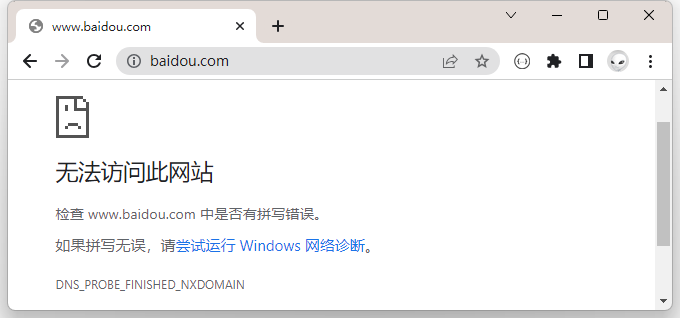
\includegraphics[width=0.5\linewidth]{figures/url404}
\end{figure}


%% ============= 8
\item 答案:D。数据库操作步骤:① 建立数据库连接\lstinline|db=sqlite3.connect("数据库文件名")|;② 建立读写游标\lstinline|cur=db.cursor()|;③ 执行SQL语句\lstinline|cur.execute("SQL语句")|;④若修改则提交\lstinline|db.cursor()|,若查询则获取数据\lstinline|db.fetchall()|;⑤关闭游标\lstinline|cur.close()|,再关闭连接\lstinline|db.close()|。

%% ============= 9
\item 考查信息系统搭建的应用:
	\begin{enumerate}[label=$(\arabic*)$]
	\item 数据采集与传输,考查题目情景和数据的理解,Python文本文件操作相关应用。
\setcounter{qnumber}{1}
\begin{lstlisting}[numbers=left]
f = open("pm_d.txt") 					# 打开文件
def finds(c, st):						# 查找字符st在字符串c中的位置
    for i in range(len(c)):
        if `\clozeblank{2}`:
            return i
data = [];  sum = 0
for line in f.readlines():			    # 按行读取文件
    if "PM2.5" in line:
        w = finds(line, " : ")
        d = `\clozeblank{2}`
        data = data + [d] 				# 将获取的 PM2.5数据保存到列表中
        sum = sum + d 
ave = - sum / len(data) 				# 计算PM2.5的平均值
# 计算AQI, 代码略
f.close()
\end{lstlisting}
		\begin{enumerate}[label=$(\alph*)$]
		\item 第①题要注意的题目设问的是“PM2.5”的平均值,这并不是前3行数据,而是第1、4、7行数据的平均值。
		\item 由第2行的注释,st是待查找字符,因此第4行程序\lstinline|c[i] == st|。
		\item 第7行程序遍历了数据文件中的每行字符串,第8行表示这行包含了“PM2.5”字符串,第9行程序找到了字符“:”所在的位置,因此第10程序截取的数值位置应该从$w+1$开始,答案是\lstinline|int(line[w+1:])|。
		\end{enumerate}	
\setcounter{qnumber}{1}
\begin{lstlisting}[numbers=left]
from flask import Flask, render_template, request
app = Flask(__name__)
# 数据处理子程序上传的AQI数据,并存储到数据库data.db的路由(代码略)
`\clozeblank{2}` 	  	 # 主页面路由命令
def index():
    db = sqlite3.connect("data.db")
    # 游标变量cur连接等参数,代码略
    sql = "SELECT * FROM pm_b WHERE id=4"
    cur.execute(sql)         # 查询4号监测点AQI数据
    data = cur.fetchall()
    # 数据库执行和关闭,代码略
    return data              # 将data数据传递给参数变量s用于显示在网页中
if __name__ == "__main__":
    app.run(`\clozeblank{2}`)
\end{lstlisting}
	\item 数据存储与呈现。考查Flask、sqlite3数据库操作。
		\begin{enumerate}[label=$(\alph*)$]
		\item 第4行程序定义路由地址,第5行定义相应的视图函数。主页的地址只需写“/”,答案是\lstinline|@app.route("/")|,除“/”地址外,其他都是固定格式,请记牢。
		\item 第6行程序连接了数据库文件“data.db”,注意这不是数据表,数据表是数据库中的一张表格。由第8行SQL语句知,数据表名称是“pm\_b”,认识这个必须要认识数据库操作的四个操作语句“SELECT”、“INSERT INTO”、“DELETE FROM”、“CREATE TABLE”。第9行程序执行了sql语句后,第10行程序可以读取到pm\_b数据表中的所有数据。
		\item 第14行,app.run()函数的格式是固定的,它一般有两个参数:host参数指明服务器地址,若省略则是IP地址“127.0.0.1”,若是“0.0.0.0”则表示服务器上当前生效的IP地址(这一般再架构图或题干中会已知)。另一个参数是port,表示端口号。注意指明host的值应该是IP地址,不需要http协议,更不需要冒号+端口号。所以答案是B。
		\item 由第10行程序知,data变量保存了数据表中的数据,现在要将它传递给网页变量$s$,那么赋值格式应该是\lstinline|s = data|,因此答案是\lstinline|render_template("index.html", s=data)|,选D。
		\end{enumerate}	
	\end{enumerate}


\end{enumerate}


\newpage

%\chapter{综合练习}\index{综合练习}
\section{综合练习一}\index{综合练习一}

\begin{enumerate}
%% ============= 1
\item 答案:B。

%% ============= 2
\item 答案:C。

%% ============= 3
\item 答案:A。

%% ============= 4
\item 答案:B。

%% ============= 5
\item 答案:A。

%% ============= 6
\item 答案:D。

%% ============= 7
\item 答案:D。

%% ============= 8
\item 答案:D。

%% ============= 9
\item 考查信息系统搭建的应用:
	\begin{enumerate}[label=$(\arabic*)$]
	\item 数据采集与传输,考查题目情景和数据的理解,Python文本文件操作相关应用。
\setcounter{qnumber}{1}
\begin{lstlisting}[numbers=left]
f = open("pm_d.txt") 					# 打开文件
def finds(c, st):						# 查找字符st在字符串c中的位置
    for i in range(len(c)):
        if `\clozeblank{2}`:
            return i
data = [];  sum = 0
for line in f.readlines():			    # 按行读取文件
    if "PM2.5" in line:
        w = finds(line, " : ")
        d = `\clozeblank{2}`
        data = data + [d] 				# 将获取的 PM2.5数据保存到列表中
        sum = sum + d 
ave = - sum / len(data) 				# 计算PM2.5的平均值
# 计算AQI, 代码略
f.close()
\end{lstlisting}
		\begin{enumerate}[label=$(\alph*)$]
		\item 第①题要注意的题目设问的是“PM2.5”的平均值,这并不是前3行数据,而是第1、4、7行数据的平均值。
		\item 由第2行的注释,st是待查找字符,因此第4行程序\lstinline|c[i] == st|。
		\item 第7行程序遍历了数据文件中的每行字符串,第8行表示这行包含了“PM2.5”字符串,第9行程序找到了字符“:”所在的位置,因此第10程序截取的数值位置应该从$w+1$开始,答案是\lstinline|int(line[w+1:])|。
		\end{enumerate}	
\setcounter{qnumber}{1}
\begin{lstlisting}[numbers=left]
from flask import Flask, render_template, request
app = Flask(__name__)
# 数据处理子程序上传的AQI数据,并存储到数据库data.db的路由(代码略)
`\clozeblank{2}` 	  	 # 主页面路由命令
def index():
    db = sqlite3.connect("data.db")
    # 游标变量cur连接等参数,代码略
    sql = "SELECT * FROM pm_b WHERE id=4"
    cur.execute(sql)         # 查询4号监测点AQI数据
    data = cur.fetchall()
    # 数据库执行和关闭,代码略
    return data              # 将data数据传递给参数变量s用于显示在网页中
if __name__ == "__main__":
    app.run(`\clozeblank{2}`)
\end{lstlisting}
	\item 数据存储与呈现。考查Flask、sqlite3数据库操作。
		\begin{enumerate}[label=$(\alph*)$]
		\item 第4行程序定义路由地址,第5行定义相应的视图函数。主页的地址只需写“/”,答案是\lstinline|@app.route("/")|,除“/”地址外,其他都是固定格式,请记牢。
		\item 第6行程序连接了数据库文件“data.db”,注意这不是数据表,数据表是数据库中的一张表格。由第8行SQL语句知,数据表名称是“pm\_b”,认识这个必须要认识数据库操作的四个操作语句“SELECT”、“INSERT INTO”、“DELETE FROM”、“CREATE TABLE”。第9行程序执行了sql语句后,第10行程序可以读取到pm\_b数据表中的所有数据。
		\item 第14行,app.run()函数的格式是固定的,它一般有两个参数:host参数指明服务器地址,若省略则是IP地址“127.0.0.1”,若是“0.0.0.0”则表示服务器上当前生效的IP地址(这一般再架构图或题干中会已知)。另一个参数是port,表示端口号。注意指明host的值应该是IP地址,不需要http协议,更不需要冒号+端口号。所以答案是B。
		\item 由第10行程序知,data变量保存了数据表中的数据,现在要将它传递给网页变量$s$,那么赋值格式应该是\lstinline|s = data|,因此答案是\lstinline|render_template("index.html", s=data)|,选D。
		\end{enumerate}	
	\end{enumerate}


\end{enumerate}


\newpage







\end{document} 